\documentclass[border=10pt]{standalone}
\usepackage[svgnames]{xcolor}
\usepackage{amsmath}
\usepackage{pgfplots}
\pgfplotsset{compat=newest}
\usepackage[sfdefault]{FiraSans}
\usepackage{FiraMono}
\renewcommand*\familydefault{\sfdefault}
\begin{document}
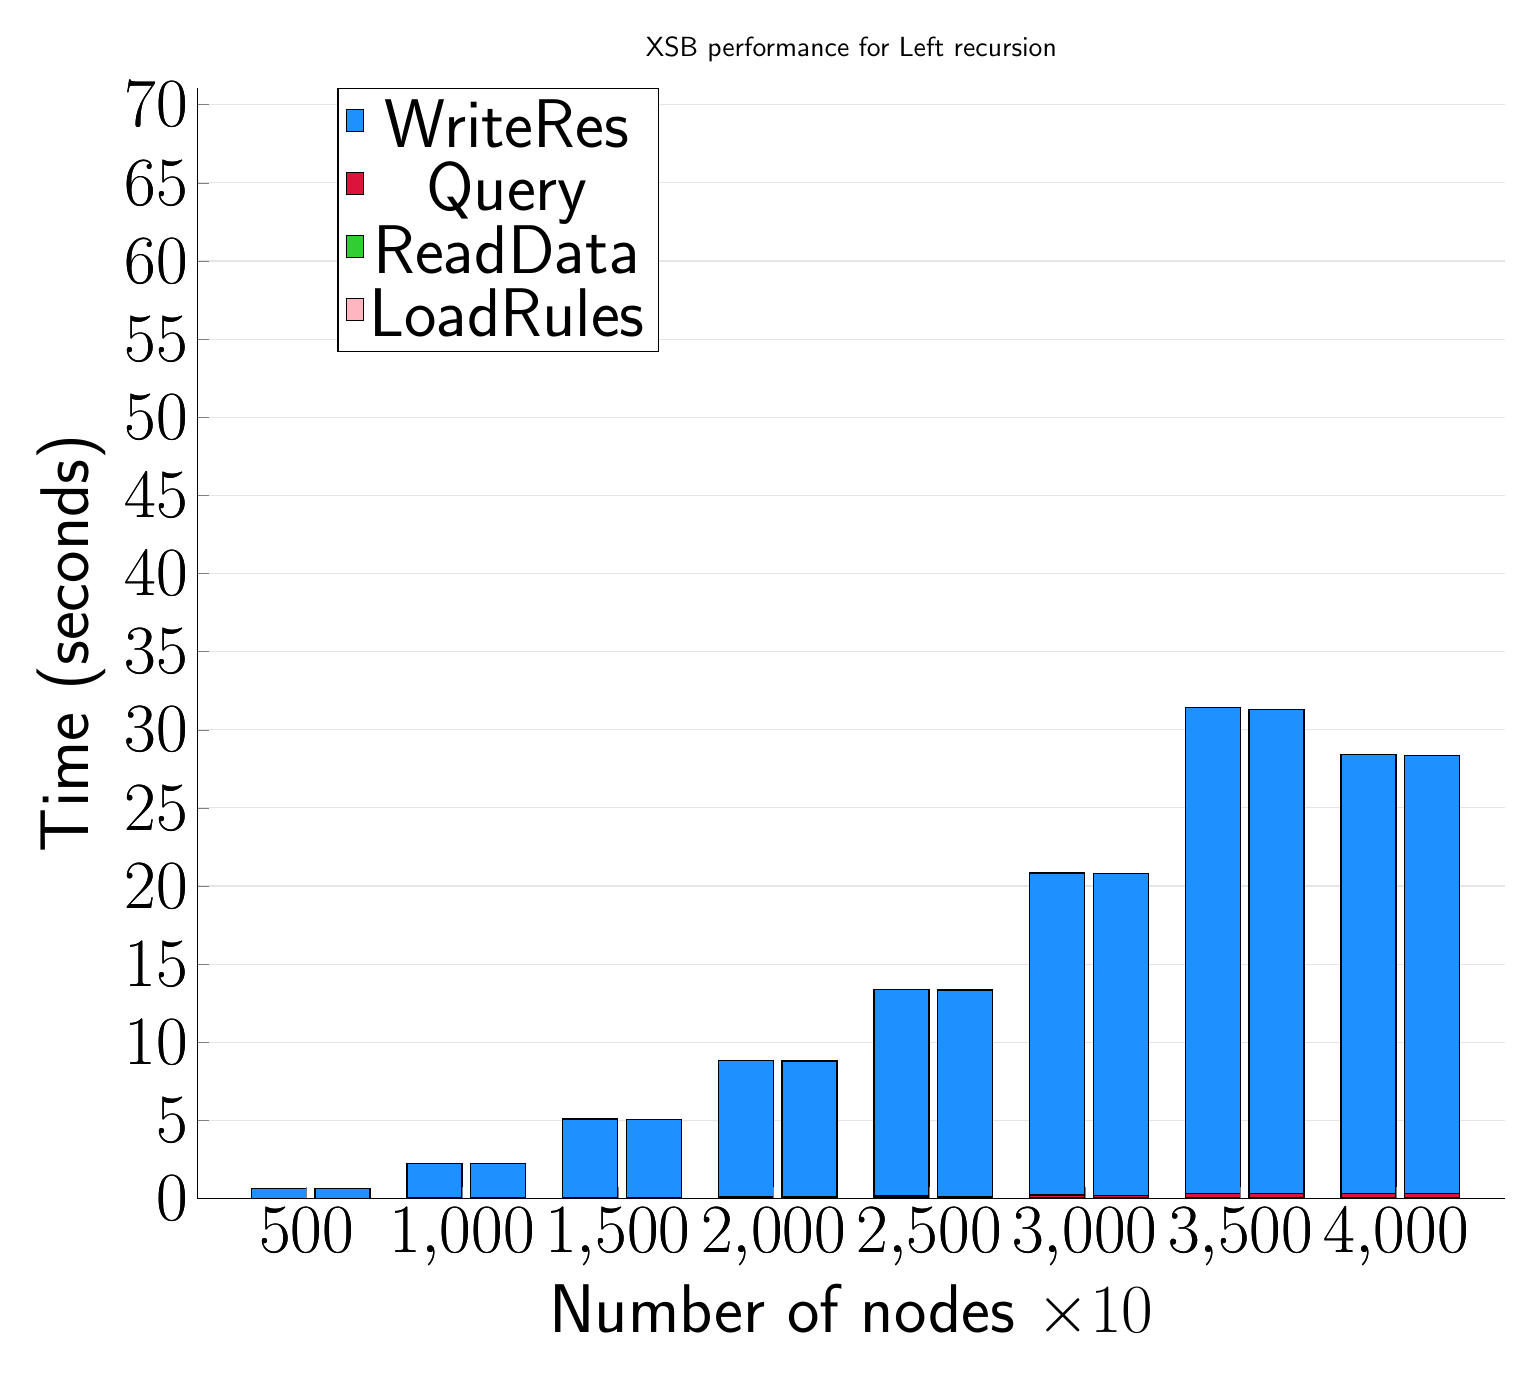
\begin{tikzpicture}
\begin{axis}[
   ybar stacked,
   title={XSB performance for Left recursion},
   bar shift=-10pt,
   width=1.5\textwidth,
   bar width=0.7cm,
   ymajorgrids, tick align=inside,
   major grid style={draw=gray!20},
   xtick=data,
   ymin=0, ymax=71.079008658727,
   axis x line*=bottom,
   axis y line*=left,
   enlarge x limits=0.1,
   legend style={
       at={(0.23, 1)},
       anchor=north,
       legend columns=1,
       font=\Huge,
   },
   ylabel={Time (seconds)},
   xlabel={Number of nodes $\times 10$},
   label style={font=\Huge},
   tick label style={font=\Huge},
]
\addlegendimage{fill=DodgerBlue, draw=black, line width=0.2pt}
\addlegendentry{WriteRes}
\addlegendimage{fill=Crimson, draw=black, line width=0.2pt}
\addlegendentry{Query}
\addlegendimage{fill=LimeGreen, draw=black, line width=0.2pt}
\addlegendentry{ReadData}
\addlegendimage{fill=LightPink, draw=black, line width=0.2pt}
\addlegendentry{LoadRules}
\addplot +[fill=LightPink, draw=black, line width=0.5pt] coordinates {
    (500, 0.0054926872253418)
    (1000, 0.004994392395019534)
    (1500, 0.004615942637125653)
    (2000, 0.004798332850138343)
    (2500, 0.004564921061197917)
    (3000, 0.005111376444498699)
    (3500, 0.005009015401204427)
    (4000, 0.003990729649861653)
};
\addplot +[fill=LimeGreen, draw=black, line width=0.5pt] coordinates {
    (500, 0.010308663050333657)
    (1000, 0.016203959782918304)
    (1500, 0.023581345876057966)
    (2000, 0.029669682184855165)
    (2500, 0.037089029947916664)
    (3000, 0.042407035827636726)
    (3500, 0.05591130256652833)
    (4000, 0.0502126216888428)
};
\addplot +[fill=Crimson, draw=black, line width=0.5pt] coordinates {
    (500, 0.0046890576680501325)
    (1000, 0.017491658528645832)
    (1500, 0.0463254451751709)
    (2000, 0.0714542865753174)
    (2500, 0.12755632400512698)
    (3000, 0.169878641764323)
    (3500, 0.266693671544393)
    (4000, 0.27127234141031903)
};
\addplot +[fill=DodgerBlue, draw=black, line width=0.5pt] coordinates {
    (500, 0.6135121981302896)
    (1000, 2.2120047410329176)
    (1500, 5.007858276367189)
    (2000, 8.729068120320635)
    (2500, 13.210900783538806)
    (3000, 20.622248093287144)
    (3500, 31.07900865872701)
    (4000, 28.11195365587871)
};
\end{axis}
\begin{axis}[
   ybar stacked,
   bar shift=13pt,
   width=1.5\textwidth,
   bar width=0.7cm,
   ymajorgrids, tick align=inside,
   major grid style={draw=none},
   xtick=data,
   ymin=0, ymax=71.079008658727,
   axis x line*=none,
   axis y line*=none,
   enlarge x limits=0.1,
   label style={font=\Huge},
   tick label style={font=\Huge},
]
\addplot +[fill=LightPink, draw=black, line width=0.5pt] coordinates {
    (500, 0.0049440000000000005)
    (1000, 0.004467666666666673)
    (1500, 0.0033053333333333303)
    (2000, 0.004451666666666664)
    (2500, 0.004563)
    (3000, 0.0044863333333333335)
    (3500, 0.004998333333333337)
    (4000, 0.0037359999999999997)
};
\addplot +[fill=LimeGreen, draw=black, line width=0.5pt] coordinates {
    (500, 0.010025999999999998)
    (1000, 0.015916666666666666)
    (1500, 0.023359)
    (2000, 0.029436)
    (2500, 0.03692566666666667)
    (3000, 0.04203833333333334)
    (3500, 0.055746)
    (4000, 0.04949633333333334)
};
\addplot +[fill=Crimson, draw=black, line width=0.5pt] coordinates {
    (500, 0.003293333333333337)
    (1000, 0.014888666666666666)
    (1500, 0.03638333333333333)
    (2000, 0.07140866666666668)
    (2500, 0.11055366666666666)
    (3000, 0.1566753333333333)
    (3500, 0.25434066666666666)
    (4000, 0.261251)
};
\addplot +[fill=DodgerBlue, draw=black, line width=0.5pt] coordinates {
    (500, 0.6094946666666666)
    (1000, 2.214624)
    (1500, 5.005539)
    (2000, 8.701642000000001)
    (2500, 13.194564666666666)
    (3000, 20.590858333333333)
    (3500, 31.00154466666667)
    (4000, 28.023601)
};
\end{axis}
\end{tikzpicture}

\end{document}
